In this section we define the specific measurements, data analysis and relationships for the framework to to meet the objectives of quantifying comprehension effort as related to interest payments on technical debt.

Data for calculating the comprehension effort for developers comes from the $Blaze$~\cite{Snipes_etal:2014} monitoring tool.  $Blaze$ logs events anonymously from developer actions in Visual Studio including menu commands, shortcut-keys, and source code editor actions such as moving the insertion carat and scrolling.  Table~\ref{fig:SampleEventData} shows a sample of the log data where each row contains a date and time (date not shown) for the event, a unique ID anonymously assigned to the developer, the event name recorded from Visual Studio, and a reference to the source file and location within the file.

\begin{table}
	\centering
	\caption{Sample Data From Event Log}
	\begin{tabular}{|l|l|l|l|}
	\hline

Time-stamp & User & Event & Artifact \\
\hline\hline
22:04:51 & N3 & View.SourceFile & 1acc7366.cs/10 \\
\hline
22:04:52 & N3 & View.OnChangeCaretLine & 1acc7366.cs/14 \\
\hline
22:04:53 & N3 & View.OnChangeCaretLine & 1acc7366.cs/16 \\
\hline
22:04:58 & N3 & Menu.ViewCallHierarchy & 1acc7366.cs/16 \\
\hline
22:05:00 & N3 & View.OnChangeCaretLine & 1acc7366.cs/20 \\
\hline
22:05:19 & N3 & View.SourceFile & 81c2db1a.cs/1 \\
\hline
22:05:22 & N3 & Edit.Find & 81c2db1a.cs/1 \\
\hline
22:05:30 & N3 & Edit.FindNext & 81c2db1a.cs/20 \\
\hline

	\end{tabular}
%	\includegraphics[width=2.75in]{figures/SampleEventData.pdf}
	\label{fig:SampleEventData}
\end{table}

Measuring comprehension effort from $Blaze$ monitoring logs requires extracting development sessions from the data that segment the stream of activity into periods where the developer is focused on a particular class.  We define a session as fixed length time window where the developer is investigating a certain class we call the central class.  The session time window begins with the first time the developer visits a certain class and ends with the last occurrence of a visit to the class within the fixed length time window.  The length of the time window is a variable we investigate in Section \ref{sec:AnalysisResults}.  
\Comment{Will:I think the previous 3 sentences define what we call a super block in our discussions}
\Fix{Will:See AnalysisResults question about number of sessions and consider moving the paragraph with that information here.}

Within a session, we calculate measurements related to comprehension effort as follows:
\begin{itemize}
	\item[] $Number of sessions$ is the number of time window sessions formed by each class 
	\item[] $Count Number of Class Visits$ is the number of times the class itself has been accessed inside a session \Fix{Will:changed Edits to Visits..I think we mean visits?}
	\item[] $Count Number of Other Class Accesses$ is the number of unique files visited in each session
	\item[] $Time Spent in Class$ is the time spent in the class that forms the session
	\item[] $Time Spent in Other Classes$ is the time spent in all other files in the session
\end{itemize}

\Fix{The following is unclear in the context of block and super block}
When sessions repeat, additional or fewer classes may be viewed by the developer, regardless they incur some comprehension effort which we add to the interest payments.  In each session, we determine the interest amount from the comprehension data quantifying it in hours. 

In Figure \ref{fig:SessionDataConcept} we show the session concept.  The session starts with the first visit to Class A under the green circle.  After that other classes C and E are visited including a visit to Class A again before the last visit to Class A under the red hexagon.  After the last visit the session time window expires.  The next session starts with a visit to Class A that begins a new 4 hour window.  In this visit classes C and E are visited as well before the developer returns to Class A.  Thus you see there are two sessions for Class A which contain a total of five visits to Class A, three visits to Class C and two visits to Class E.
\begin{figure}
	\centering
	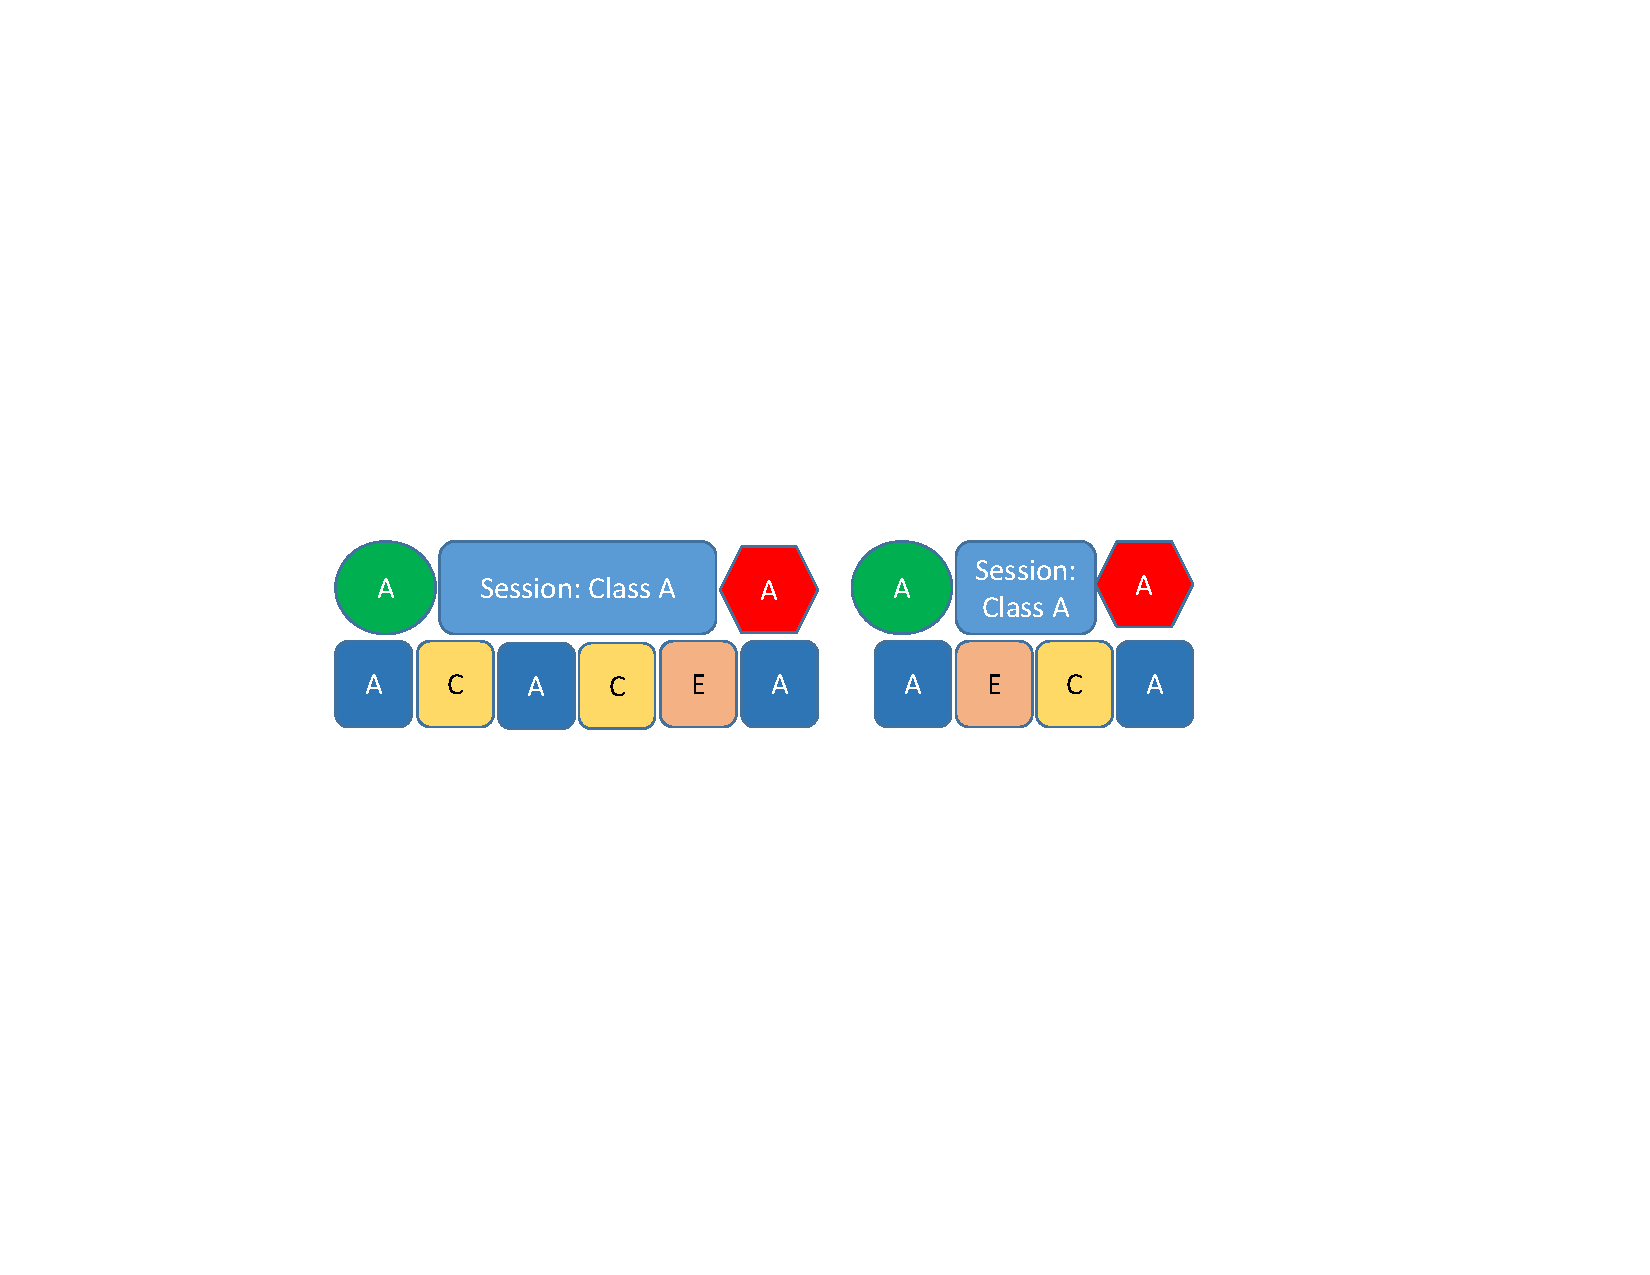
\includegraphics[width=3in]{SessionDataConcept.pdf}
	\caption{Conceptual View of Sessions}
	\label{fig:SessionDataConcept}
\end{figure}

Developers at ABB volunteered to install $Blaze$ and record their actions in Visual Studio.  The data set evaluated for this study focuses on two developers with more than 3 months of data.  Because the data are anonymous, we have no demographic information on the developers to characterize their experience or knowledge.

The framework matches the comprehension data with code structure data at the class level.  Therefore we consider class level code structure metrics whose definitions align with the measurements taken for comprehension.  Data for code structure is provided by the $Understand$ tool from Scientific Tool Works.  The framework used the following metrics for code structure data at the class level:

\begin{itemize}
	\item[] $Count Class Coupled$ is the number of other classes coupled to
	\item[] $Count Class Base$ is the Number of immediate base classes
	\item[] $Count Class Derived$ is the number of immediate sub-classes
	\item[] $Count Declared Method$ is the number of local methods for the class
\end{itemize}

The class level metrics for code structure are related to comprehension metrics through the name of the source file in the $Blaze$ data corresponding to the class.  In cases where the source file contains multiple classes, the structure metrics were aggregated.

Aligning these two data sources at the module level allows us to ask questions of the intersected data set.  For example, we find the following questions interesting:

\begin{itemize}
	\item[] How much time does the developer spend understanding the code related to the change they are making?
	\item[] How many code elements does the developer need to review related to the change?
	\item[] How many dependent classes does the developer need to review related to the change?
	\item[] How correlated are comprehension effort metrics with code structure metrics?
	\item[] As code structure metic values change, is the corresponding change in comprehension effort linear or non-linear.
\end{itemize}